

\section{AO-GPT: a Decoder-only Model with the Potential to Unify AR and MDM} 
\label{sec:model}

\subsection{Significance and Future Potential}
We highlight here its broader significance and future potential. The development of efficient and effective decoder-only MDMs like AO-GPT is crucial for several reasons:

\textbf{Broader Scope:} Firstly, the strong left-to-right sequentiality inherent in natural language, which often favors standard autoregressive (AR) models, may not be as pronounced in other discrete data modalities. For domains such as biological sequences, symbolic music, or certain structured code representations, the inherent flexibility of an any-order AR approach could be more naturally suited. Implementing such models within a decoder-only architecture, as AO-GPT proposes, could offer substantial advantages over rigidly ordered AR models, potentially leading to more effective modeling and generation in these diverse fields.

\textbf{Efficiency:} Secondly, within the realm of language modeling itself, the pursuit of decoder-only MDMs is driven by a compelling trade-off between modeling paradigms and computational efficiency. Decoder-only AO-AR offers significant theoretical and empirical advantages in density estimation and generation in terms of theoretical computational complexity and empirical generation speed (as discussed in Section~\ref{sec:decoupling}, \ref{sec:mdm encoder decoder} and indicated by Finding 7, 8.1).

\textbf{Flexibility:} Thirdly, decoder-only AO-AR frameworks like AO-GPT exhibit superior flexibility in controlling the distribution over token generation orders. While encoder-only AO-AR models can vary the distribution of the number of masked tokens, they cannot easily specialize to a strict, fixed-order autoregressive model (e.g., left-to-right). In contrast, decoder-only AO-AR models can directly learn from any permutation distribution $P(S_n)$. This allows them to instantiate a standard left-to-right AR model by simply using the identity permutation ($\sigma = \text{id}$), or to train on hybrid order distributions (as shown in Section~\ref{sec:decoder ar vs mdm}). This adaptability uniquely positions them to interpolate between, and potentially unify, autoregressive and masked diffusion paradigms within a single architecture.



\subsection{Injecting Target Position Information}
In this section, we will give a comprehensive description of the modeling details, training, and inference of masked diffusion models using a decoder-only architecture. To train autoregressive models on sequences in \textit{any order} with a decoder-only model, a key architectural modification is necessary compared to standard GPT: adding explicit \textit{target position} information. In a traditional AR model setup (like GPT), the model implicitly predicts the token immediately succeeding the current one; the target position is always the next index in the sequence. 

However, when processing sequences in a shuffled order according to a permutation $\sigma = (\sigma_1, \dots, \sigma_n)$, the token at step $t$ in the shuffled sequence is $\boldsymbol{x}_{\sigma_t}$, and the target token to predict at step $t$ is $\boldsymbol{x}_{\sigma_{t+1}}$. The original position $\sigma_{t+1}$ is not fixed relative to the current step $t$, but varies depending on the specific permutation. Therefore, at step $t$, to predict $\boldsymbol{x}_{\sigma_{t+1}}$, the model should access the information of the input representation for tokens $\boldsymbol{x}_{\sigma_{\leq t}}$, its position in the original sequence ($\sigma_{\leq t}$), and crucially, the original position $\sigma_{t+1}$ of the next token to be predicted in the shuffled sequence. This is necessary because transformers need the explicit target original position ($\sigma_{t+1}$) to identify which specific original position's token it should predict next, a requirement absent in fixed-order prediction.

We identify two existing decoder-only architectures for training order-agnostic autoregressive models: XL-Net~\cite{yang2019xlnet} and $\sigma$-GPT~\cite{pannatier2024sigma}. XL-Net incorporates the target position using two-stream attention, a mechanism that differs significantly from mainstream decoder architectures. Therefore, we do not adopt this approach. In contrast, $\sigma$-GPT incorporates the target position through an additional target positional encoding on a standard GPT architecture as~\Cref{fig:target inject}(a). Thus, we choose to adopt $\sigma$-GPT as a baseline method.


\subsection{Design Space of AO-GPT}
\begin{figure}[t]
  \centering
  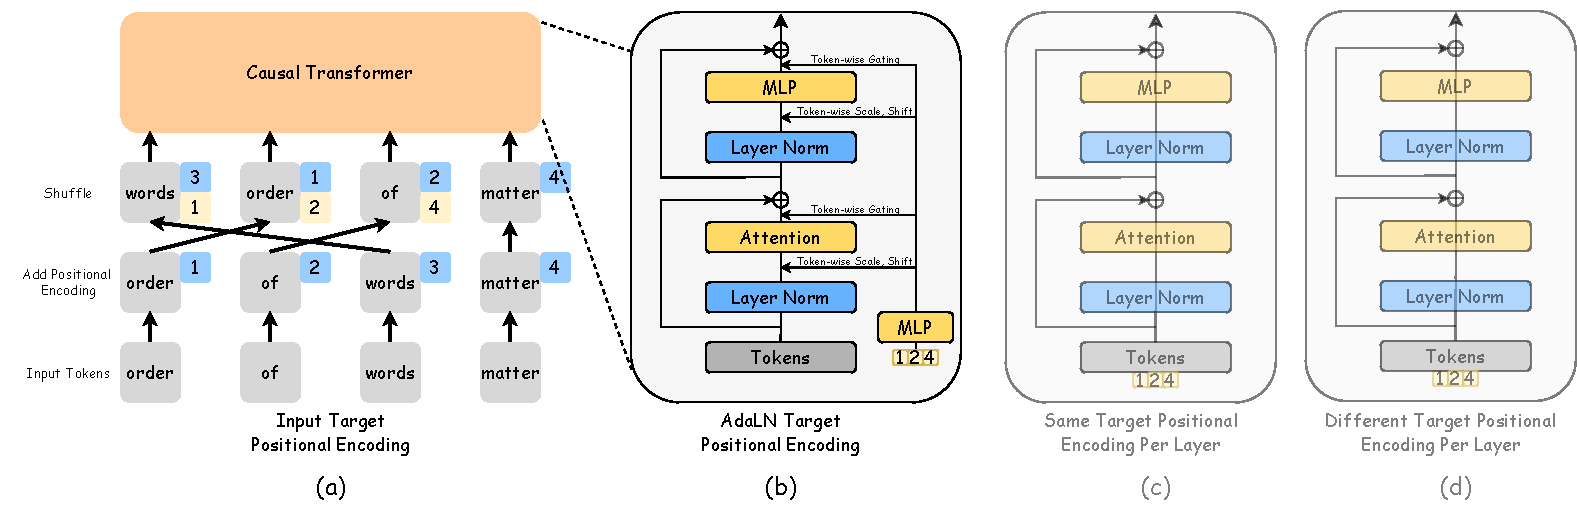
\includegraphics[width=1.0\linewidth]{plots/model_architecture_variants_v2.drawio.pdf}
  \caption{Target position injection strategies for decoder-only AO-AR model.}
  \label{fig:target inject}
\end{figure}


\begin{figure}[t]
    \centering 

    \begin{subfigure}[b]{0.5\linewidth}
        \centering 
        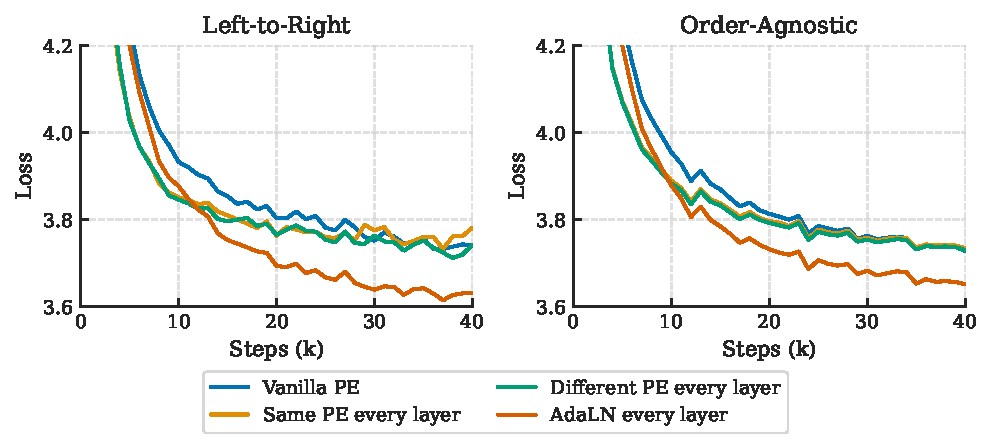
\includegraphics[width=\linewidth]{plots/ablate_pe.pdf} 
        \caption{Ablation on Target Position Injection}
        \label{fig:ablate_pe} 
    \end{subfigure}%
    \begin{subfigure}[b]{0.5\linewidth}
        \centering
        % 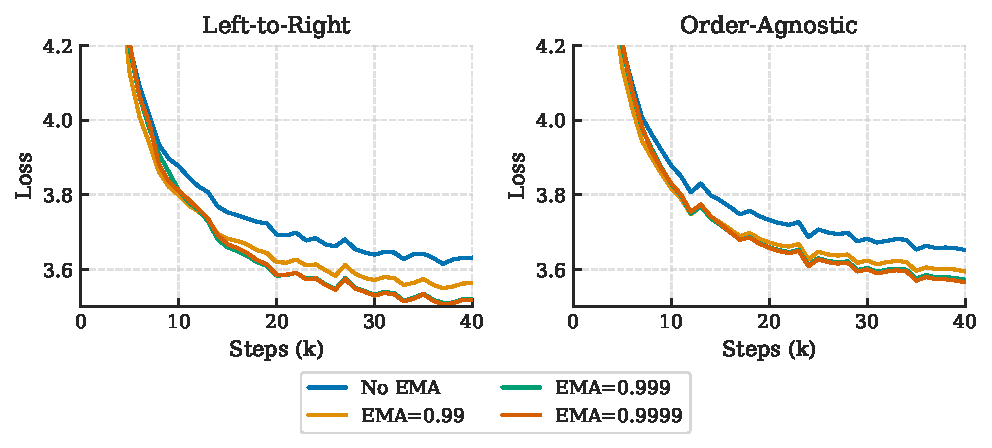
\includegraphics[width=\linewidth]{plots/ablate_ema.pdf}
        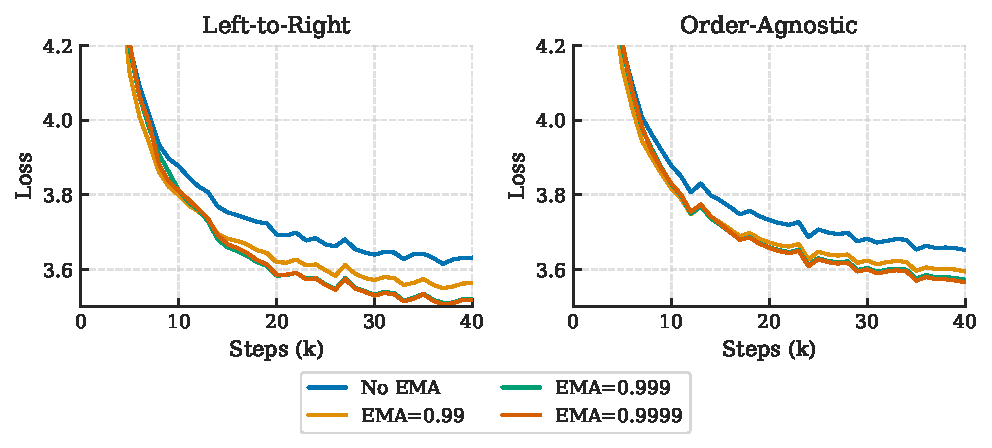
\includegraphics[width=\linewidth]{plots/ablate_ema.pdf} 
        \caption{Ablation on Exponential Moving Average (EMA)}
        \label{fig:ablate_ema}
    \end{subfigure}
    \caption{Ablation studies for AO-GPT: target positional encoding and exponential moving average.}
    \label{fig:ablation_combined}
\end{figure}
\subsubsection{Target Position Injections}


We observe slow convergence in $\sigma$-GPT, particularly during its initial training stages. Beyond the factors analyzed in~\Cref{sec:decoder ar vs mdm}, we hypothesize that the semantic requirements imposed by the target position significantly influence the predicted token, potentially more so than a simple target position encoding can adequately capture. For instance, in the sentence \texttt{She put the \_ in the \_}, the first blank typically requires a noun representing a movable object (e.g., \texttt{book, key, food}), while the second necessitates a noun denoting a container or location (e.g., \texttt{box, drawer, fridge}). The distinct lexical distributions for these two positions suggest that a single, undifferentiated target position encoding applied after the token embedding may be insufficient to model these nuanced, position-dependent semantic constraints.

To address this potential limitation, we propose and ablate three distinct strategies for incorporating richer target position information, all designed to incur negligible additional computational cost: (1)~\Cref{fig:target inject}(c) re-applying the same target positional encoding at the input of each Transformer block; (2)~\Cref{fig:target inject}(d) utilizing distinct, learnable target positional encodings for each Transformer block; and (3)~\Cref{fig:target inject}(b) conditioning the LayerNorm parameters~\cite{perez2018film,peebles2023scalable} within each Transformer block on the target position. As shown in~\Cref{fig:ablation_combined}, the former two ways demonstrate some early training acceleration compared to the baseline, but their advantages diminish in later stages, eventually performing nearly identically to the baseline. In contrast, the adaptive LayerNorm (adaLN) approach shows consistent improvements throughout the entire training process. This suggests that dynamically modulating LayerNorm parameters based on target position provides a more effective and stable way to incorporate positional information, likely because it allows for finer-grained, context-dependent normalization at each transformer block.


\subsubsection{Exponential Moving Average}

While Exponential Moving Average (EMA) of model weights is a less common technique in the pre-training of standard autoregressive language models, it is a widely adopted practice in the training of both continuous and current discrete diffusion models, where it often contributes to improved sample quality and training stability.
Given the potential for EMA to smooth the training trajectory, and potentially to help smooth out
noise, allowing the optimization to converge to the target loss more efficiently, we conducted an ablation study to assess its impact on OA-GPT. We experimented with several EMA decay rates: 0.99, 0.999, and 0.9999, comparing these against a baseline model trained without EMA. Our results indicate a clear benefit to employing EMA. All tested EMA configurations outperformed the baseline model (no EMA). Notably, an EMA decay rate of 0.9999 yielded the best performance among the values tested.


\begin{figure}[t]
  \centering
  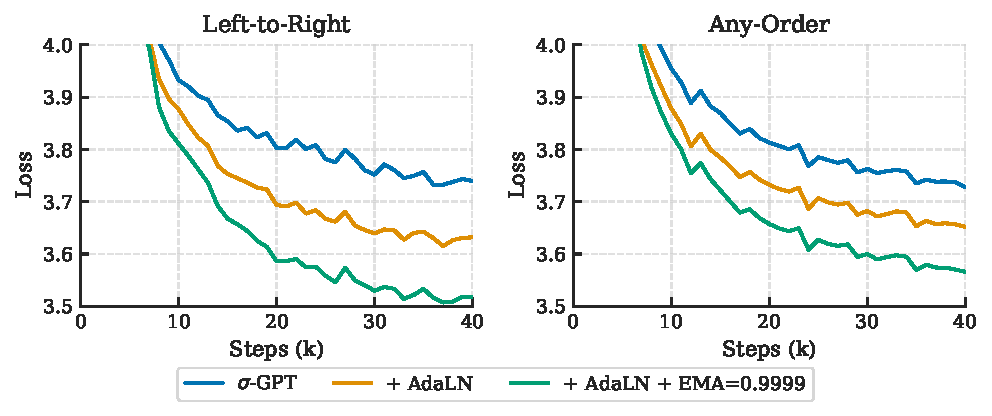
\includegraphics[width=1.0\linewidth]{plots/ablate_all.pdf}
  \caption{Combined impact of adaptive layerNorm (AdaLN) and exponential moving average (EMA) on AO-GPT training. Loss curves compare the baseline $\sigma$-GPT, $\sigma$-GPT with AdaLN, and $\sigma$-GPT with both AdaLN and EMA (decay 0.9999) for Left-to-Right (left) and Any-Order (right) objectives.}
  \label{fig:compare sigma ao}
\end{figure}

\begin{table}\small
  \caption{Zero-shot validation perplexity($\downarrow$) on a variety of datasets on GPT-2-medium sized models ($\sim$350M). $^\dagger$Model reproduced by the authors. $^\ddagger$Model trained with an additional 10\% left-to-right ordered data.}
  \label{tab:compare sigma ao}
  \centering
  \begin{tabular}{@{}l ccccc@{}}
    \toprule
    \textbf{Model} & \textbf{LAMBADA} & \textbf{WikiText2} & \textbf{PTB} & \textbf{WikiText103} & \textbf{1BW} \\
    \midrule

    % --- Encoder-only Models ---
    \multicolumn{6}{@{}l}{\textit{Left-to-Right}} \\ % Header spans all 6 columns
    \quad\quad $\sigma$-GPT$^\dagger$ &61.05 &44.80 &121.48&43.68&76.74\\
    \quad\quad \textit{AO-GPT$^\ddagger$}&\textbf{42.44} &\textbf{31.52}&\textbf{87.56}&\textbf{30.86}& \textbf{50.23} \\
    \midrule % Separator between major categories
    \multicolumn{6}{@{}l}{\textit{Any-Order}} \\
    % \addlinespace % Optional extra space
    \quad\quad $\sigma$-GPT$^\dagger$  &57.27 &43.28&126.11 &41.80 & 74.81 \\
    \quad\quad \textit{AO-GPT$^\ddagger$}  &\textbf{49.79}&\textbf{33.73}&\textbf{101.01} &\textbf{32.38}&\textbf{65.90}\\
    \bottomrule
  \end{tabular}
\end{table}

Having established the individual benefits of adaptive layerNorm (adaLN) for target position injection and exponential moving average (EMA) for training, we investigate their combined effect on AO-GPT. Figure~\ref{fig:compare sigma ao} illustrates the training loss progression for both Left-to-Right and Any-Order objectives when integrating both adaLN and EMA (with a decay of 0.9999) into the $\sigma$-GPT baseline. The results demonstrate that these two enhancements are largely orthogonal, with their combination leading to significantly improved convergence and lower final loss values compared to the baseline $\sigma$-GPT and models with only one of the improvements. This synergistic effect is further corroborated by the zero-shot perplexity scores presented in Table~\ref{tab:compare sigma ao}, where the fully enhanced AO-GPT (incorporating adaLN, EMA, and 10\% L2R data) substantially outperforms the reproduced $\sigma$-GPT baseline across all evaluated datasets for both Left-to-Right and Any-Order evaluations.

\subsection{Parallel Generation Attention Mask}
The reverse process in MDMs iteratively recovers masked tokens as follows:
\begin{equation}
q_{s|t} = \prod_{i=0}^{n-1} q_{s|t}(\boldsymbol{x}_s^i|\boldsymbol{x}_t),\text{where } q_{s|t}(\boldsymbol{x}_s^i|\boldsymbol{x}_t)=\begin{cases}
1, & \boldsymbol{x}_t^i \neq [\text{MASK}], \boldsymbol{x}_s^i = \boldsymbol{x}_t^i \\
\frac{s}{t}, & \boldsymbol{x}_t^i = [\text{MASK}], \boldsymbol{x}_s^i = [\text{MASK}] \\
\frac{t-s}{t} q_{0|t}(\boldsymbol{x}_s^i | \boldsymbol{x}_t), & \boldsymbol{x}_t^i = [\text{MASK}], \boldsymbol{x}_s^i \neq [\text{MASK}].
\end{cases}
\end{equation}
Here, $q_{0|t}(\boldsymbol{x}_s^i | \boldsymbol{x}_t)$ (when $\boldsymbol{x}_t^i = [\text{MASK}]$) represents a distribution over the vocabulary for predicting a non-$[\text{MASK}]$ token, provided by the model. Sampling $\boldsymbol{x}_s$ from $q_{s|t}(\boldsymbol{x}_s|\boldsymbol{x}_t)$ involves sampling each $\boldsymbol{x}_s^i$ independently. 
Crucially, AO-GPT, equipped with the specialized attention mask depicted in Figure~\ref{fig:gen attn mask}, can compute these probabilities $q_{0|t}(\boldsymbol{x}_s^i | \boldsymbol{x}_t)$ for different $i$ in a single forward pass. This mask ensures that the prediction for each masked token $\boldsymbol{x}_s^i$ is conditioned only on the unmasked tokens present in $\boldsymbol{x}_t$ and its own position, without attending to other concurrently predicted masked tokens. Consequently, this parallel prediction scheme for multiple masked tokens introduces no training/inference mismatch for the individual $q_{0|t}(\boldsymbol{x}_s^i | \boldsymbol{x}_t)$ distributions, as each is generated under conditions consistent with the model's training.

\begin{figure}[t]
  \centering
  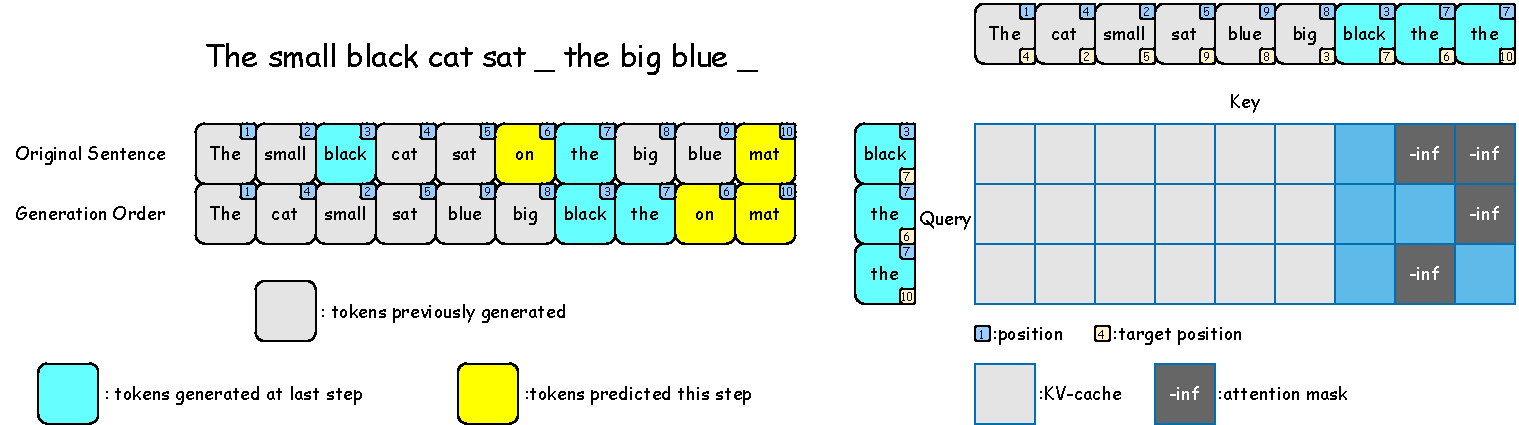
\includegraphics[width=1.0\linewidth]{plots/gen_attn_mask.drawio.pdf}
  \caption{Attention mask for simultaneous prediction of multiple tokens in AO-GPT.}
  \label{fig:gen attn mask}
\end{figure}

